\documentclass[]{article}

\usepackage{amsmath}  % AMS math package
\usepackage{amssymb}  % AMS symbol package
\usepackage{bm}       % bold math
\usepackage{graphicx} % Include figure files
\usepackage{dcolumn}  % Align table columns on decimal point
\usepackage{multirow} % Multirow/column tables
\usepackage{hyperref} % Hyperlinks
\usepackage{float}

\begin{document}

\title{2D Ising Model Representation and Analysis Using Monte Carlo and Metropolis Algorithm With Less Memory Consumption}% Force line breaks with \\
\author{Thavappiragasam Mathialakan}
\date{\today}% It is always \today, today, but you can specify other dates manually 
\maketitle

\begin{abstract}
The 2D Ising model obviously deals with mass data to study the behavior of magnetization and energy related with temperature. This analysis should be worked out in best time complexity with less memory consumption. In this paper, we introduces a less memory usage implementation technique Boolean 1D-array lattice and shows the improvement in time complexity. It also analysis this studies using our C++ coding and Matlab graphs. 
\end{abstract}


\section{Introduction} %Title for the section
\label{sec:level1} %Label for the section, to be used for referencing in other parts of the document

The electron's spin and the magnetic moment associated with are taking key role in the theory of magnetism. Ferromagnetism arises when a collection of such spins conspire so that all of their magnetic moments point in the same direction, yielding a total moment. This systems generally lose their magnetism at high temperature. The magnetic properties obviously depend on temperature. Ising model is a very useful simulation that can be used to analyze how temperature effects the magnetization.

\subsection{\label{sec:level2.1} Ising Model}
This model was proposed by Lenz (1920) to study the phase transition of ferromagnets at the Curie temperature. The one dimensional case was completely developed by his pupil (1925) and the two dimensional case was done by Onsager. This is a quantum model of a collection of spins that represent magnetic moments. Two dimensional lattice is represented in a 2D array that consists a set of spins. A spin in a lattice is in either up or down that points +z or -z.\\
The spins are considered to be interact only between the neighbors in simplest Ising model. The equation ~\ref{eq:one} express the energy of the system that is equal to sum of the all pairs of nearest neighbour spins $<i, j>$.
\begin{equation}
\label{eq:one}
E = -J \sum_{<i,j>}S_iS_j
\end{equation}

where J is the coupling constant and $S_i = \pm 1$ are the two spin states allowed in each lattice site. The energy between a single pair gives -J if tow neighbouring spins in the same direction and +J if they are antiparallel. The magnetization can be calculated by taking the sum of all spins (equation ~\ref{eq:two}). 
\begin{equation}
\label{eq:two}
M = \sum_{i}S_i
\end{equation}
The average magnetization formed by all spins is called as magnetization density. The magnetization density for a square lattice of size $N = L^2$ is given by,  
\begin{equation}
\label{eq:three}
\frac{1}{L^2} \sum_{i}S_i
\end{equation}


\subsection{\label{sec:level2.2} Monte Carlo}
The Ising model is simulated using Monte Carlo (MC) that is stochastic, nondeterministic and rely heavily on the use of random or pseudo-random numbers. MC simulations are very powerful simulations and versatile numerical tools used to study large systems. In the Ising model, the Metrapolis algorithm analysis a huge number of states/configurations. For example, There are $2^N$ considerable states in $N = L^2$ spin lattice because each spin can be either of two states. In order to avoid this inconvenience, some of the samples has been chosen from them using the MC.
The expectation value of an observable A can be given as,
\begin{equation}
\label{eq:four}
<A> = \frac{\sum_{cfg}{A_{cfg}e^{-\beta E_{cfg}}}}{\sum_{cfg}{e^{-\beta E_{cfg}}}}
\end{equation}
where $A_{cfg}$ is the value of A for the state or configuration \texttt{cfg}. So, given a system that has a discrete number of states, we could, using a computer, calculate A for each state and weight these values by their Boltzman factors to find the average A.

 One (bad) way of using random numbers would be to randomly pick a lot of states, measure A for each of them, and weight these values of A by their Boltzman factors. We might get close to the right answer if we sampled a lot of states, but we would spend a lot of time calculating A for states that contribute very little to the final result (an Ising lattice at very high temperature is unlike to be in the state with all spins pointing in one direction). Instead of sampling (measuring parameters like A for) a lot of states and then weighting them by their Boltzman factors, it makes more sense to choose states based on their Boltzman factors and to then weight them equally. This is known as the Metropolis algorithm, which is an importance sampling technique.
 
\subsection{\label{sec:level2.3} Metropolis Algorithm}
This algorithm chooses a random spin and flip it from +1 to -1 or vise versa. Due to this individual spin's flip, the energy is gained or lost, and the state is going to change from one to another. This state changing is accepted based on the energy difference of the new state related to the current state. In this way, MC simulation technique is used to fulfill the algorithm, and Boltzman factor $k_B$ is taken as 1.


\texttt{Major Steps of the Algorithm}
\begin{enumerate}
\item Set the temperature T
\item Initialize lattice
\item Do this for a given number of iterations
\begin{enumerate}
    \item Choose random spin in the lattice and flip it to opposite.
    \item Calculate the energy difference between the trial state and the present state, $\delta E$.
    \item If $\delta E \leq 0$ the trial state is accepted. Otherwise, generate a uniform random number $\delta R $ in [0, 1], and new state is accepted if $\delta R \leq e^{-\beta \delta E} $
    \item Calculate the average energy and magnetization
\end{enumerate}

\end{enumerate}

\section{Approaches to reduce memory consumption}

The lattice spin model represents set of spins in a molecular structure. A spin in a model be in one of the two states, may be up or down. This model uses a data structure 2D integer array of 1s and -1s to represent up and down spins respectively. Suppose a lattice has N spins, it has to use 32N bits of memory to keep this record. It can be reduced to N bits if we choose Boolean array. How this Boolean representation is possible? A spin is in only two possible states, so they can be represented using Boolean bi-value, true or false. The up-spin and down-spin is given by true (1) and false (0) respectively instead of 1 and -1.

This way, further of less memory usage, helps to reduce processing time using bitwise logical operations instead of time consuming arithmetic operation multiplexer (In worst case, It takes $\theta (n^2)$ to multiply two n-digit numbers ). During the energy calculation, each neighbour of a randomly selected flipped-spin is taken to multiply. A spin can has two to four neighbours or connections, but every spin has four neighbours in periodic boundary conditions, where it has link between spins in row 1, n and spins in column 1, n. 

The table ~\ref{tab:table1} shows the energy of a spin pair $<S_i, S_j>$ for all four possible combinations. The energy is doubled in a pair by the effect given to each other. This energy calculation requires two multiplication operations, $mul( mul(S_i, S_j), 2)$. In our Boolean lattice, spin pair is operated by bitwise XOR and energy is chosen to -2 or 2 based on the truth value (table ~\ref{tab:table2}). It reduces the time complexity significantly. When we are thinking in low level architecture or if we have plan to design a specific electronic controller to solve this task, deal with bitwise operation, it will support easy and very low budget project because such operations can be performed using less logic gates.   

\begin{table}
  \centering
  \begin{tabular}{ |l|l|l| }

  \hline
  \multicolumn{3}{ |c| }{Integer Representation} \\
  \hline
  $S_i$ & $S_j$ & Energy \\ \hline
  -1 & -1 & 2 \\ \hline
  -1 &  1 & -2 \\ \hline
   1 & -1 & -2 \\ \hline
   1 &  1 & 2 \\ \hline
  \end{tabular}
  \caption{\label{tab:table1}The energy of a spin pair $<S_i, S_j>$ } in integer representation
\end{table}

\begin{table}
  \centering
  \begin{tabular}{ |l|l|l|l| }

  \hline
  \multicolumn{4}{ |c| }{Boolean Representation} \\
  \hline
  $S_i$ & $S_j$ & XOR& Energy \\ \hline
   0 &  0 & 0 & 2 \\ \hline
   0 &  1 & 1 & -2 \\ \hline
   1 &  0 & 1 & -2 \\ \hline
   1 &  1 & 0 & 2 \\ \hline
  \end{tabular}
  \caption{\label{tab:table2}The energy of a spin pair $<S_i, S_j>$ } in Boolean representation
\end{table}

How to calculate the magnetization in bit/Boolean array? Suppose the lattice of size $N = L^2$ has \texttt{k} up-spins, the magnetization will be calculated by the equation ~\ref{eq:five}. In our representation, up-spins are 1 and down-spins are 0, sum of the bit array gives the number of up-spins, so the magnetization is given by the equation ~\ref{eq:six}.
\begin{equation}
\label{eq:five}
M = 2k-L^2
\end{equation}
\begin{equation}
\label{eq:six}
M = 2\sum_{i}S_i -L^2
\end{equation}

\section{Implementation}
The high-level programming language C is the most preferable language to deal with mass data, and C++ is an advanced version of C. So, we chose C to implement this ising model using Metropolis algorithm as described above. Since 1D array offers better memory locality and less allocation and deallocation overhead, It is faster way than 2D for dense matrices. As the reason given above, the data structure 1D Boolean array is chosen to keep spins in lattice.  

\section{Results and Discussion}
In our testing case, a lattice of size $N = 10^2$ is taken, and initially it is configured with all up; a 1D Boolean array of size 100 is set to true. We applied both boundary conditions (BC): 1) Every spin in all four edges of lattice has no round robin connections. 2) Periodic BC. When using the first BC, initial value of average energy and magnetization is given by $-2L(L+1)$ and 1.0 ($=L/L$) respectively. The energy will be $2N$ and the same magnetization for second BC. The average energy and magnetization are calculated for every 0.1 temperature increases in range [0, 5]. This task is processed for 10 000 iterations. The figure ~\ref{fig:Mag} shows the changes on magnetization with temperature. It decreases when temperature increases, and we found the critical temperature, $T_c$ is 2.3 approximately. The energy is a continuous function of temperature, and increases as a function of temperature (Figure ~\ref{fig:Energy}).    

\begin{figure}[h]
  \centering
  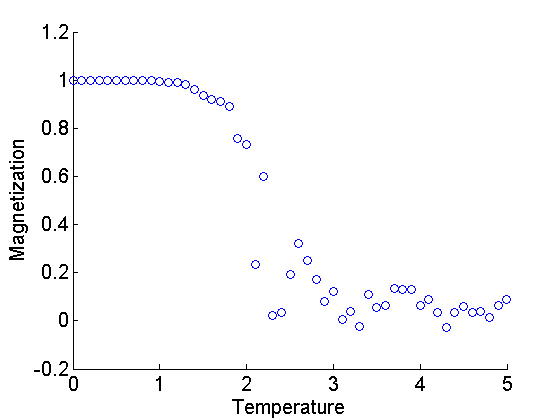
\includegraphics[width=10cm,height=8cm]{figures/Mag_Temp}
  \caption{\label{fig:Mag} The change of Magnetization with increasing temperature when $J=1$ and $k_B=1$.}
\end{figure}

\begin{figure}[t]
  \centering
  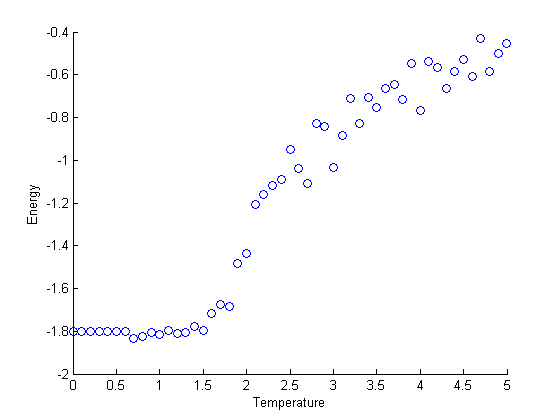
\includegraphics[width=10cm,height=8cm]{figures/Ene_temp_scatter}
  \caption{\label{fig:Energy} The change of Energy with increasing temperature when $J=1$ and $k_B=1$.}
\end{figure}

Finally, for the fixed temperature 2.3, the configuration is changed through 1000 iterations, and magnetization is measured and graphed as shown in the Figure ~\ref{fig:Config}. This falls on the linear line $y = -0.0003x + 0.9573$. And also the Figure  ~\ref{fig:Config_E} shows the energy related to configurations. The linearity of this relationship is given by the equation $y = 0.0005x - 1.6353$.

\begin{figure}[H]
  \centering
  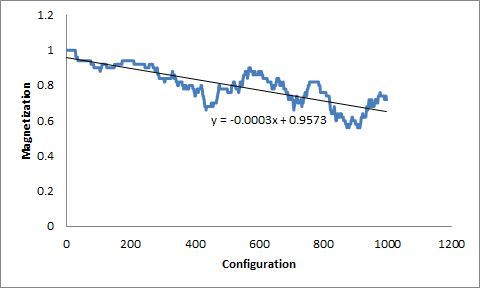
\includegraphics[width=10cm,height=6cm]{figures/Config}
  \caption{\label{fig:Config} The change of Magnetization related with configurations at temperature 2.3}
\end{figure}
\begin{figure}[H]
  \centering
  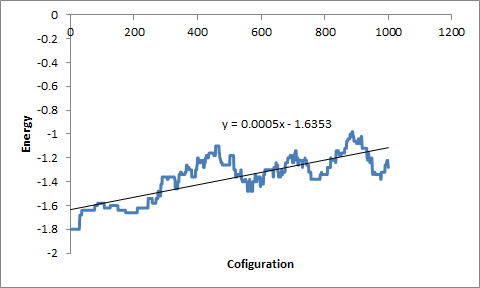
\includegraphics[width=10cm,height=6cm]{figures/Config_E}
  \caption{\label{fig:Config_E} The change of Energy related with configurations at temperature 2.3.}
\end{figure}

\section{Conclusion}
We tested our approach successfully using minimum memory and time.
The magnetization decreases with increasing temperature, but in contrast, average energy increases with it. Further, even though those measurements fluctuating for the configuration changes, It can be brought into a linear trend.
\newpage
\appendix
\section{Periodic Boundary Condition}

The figures ~\ref{fig:No_PBC} and ~\ref{fig:PBC} clearly show the distinguishes between periodic boundary condition and without it. 
\begin{figure}[H]
  \centering
  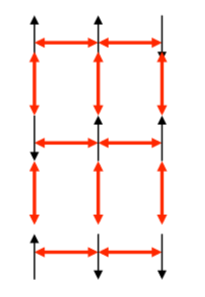
\includegraphics[width=4cm,height=6cm]{figures/NoPBC_ls}
  \caption{\label{fig:No_PBC} The links in 3x3 lattice without PBC.}
\end{figure}

\begin{figure}[H]
  \centering
  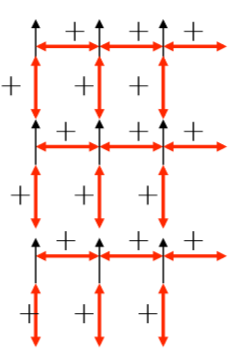
\includegraphics[width=4cm,height=6cm]{figures/PBC_ls}
  \caption{\label{fig:PBC} The links in 3x3 lattice with PBC.}
\end{figure}

We also tested our implementation of ising model for PBC, the magnetization and energy changes related with temperature are shown in figure ~\ref{fig:Mag_PBC} and ~\ref{fig:Energy_PBC}  respectively.
\begin{figure}[H]
  \centering
  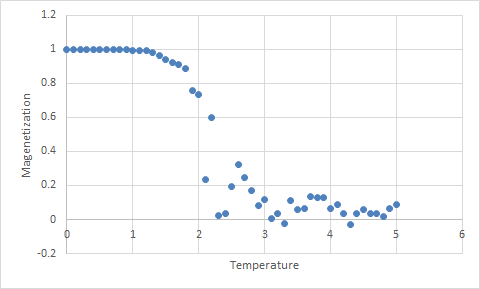
\includegraphics[width=10cm,height=6cm]{figures/Mag_Temp_PBC}
  \caption{\label{fig:Mag_PBC} The change of Magnetization with increasing temperature when $J=1$ and $k_B=1$ using PBC}
\end{figure}
\begin{figure}[H]
  \centering
  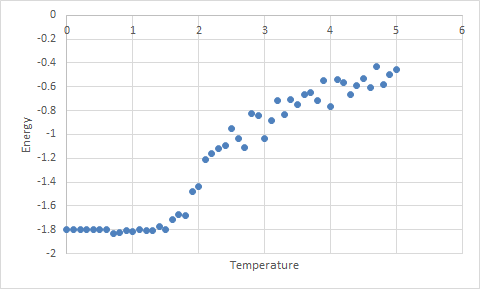
\includegraphics[width=10cm,height=6cm]{figures/Ene_temp_scatter_PBC}
  \caption{\label{fig:Energy_PBC} The change of Energy with increasing temperature when $J=1$ and $k_B=1$ using PBC}
\end{figure}

\end{document}
